\subsubsection*{Minimum drag problem}

The minimum drag problem formulated here an optimal shape
design problem with one input and one output variables, besides two boundary conditions. 
It is defined by an unconstrained objective functional requiring the integration of a function. 

Consider the design of a body of revolution with given length and diameter providing minimum drag at zero angle of attack and for neglected friction
effects. 
Figure \ref{SpaceShuttleFigure} is a picture of a space shuttle, which could be that body of revolution. 
That picture is taken from Wikipedia. 

\begin{figure}[h!]
\begin{center}
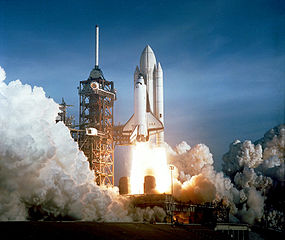
\includegraphics[width=0.7\textwidth]{optimal_shape_design/space_shuttle}
\caption{Space shuttle.}\label{SpaceShuttleFigure}
\end{center}
\end{figure}

For a slender body, the pressure coefficient can be approximated by the Newtonian flow relation.
The Newtonian flor provides us with a simple approximation for the drag.

